\chapter{Supplementary Figures}
\label{app:supplementary_figures}

This appendix presents additional figures that support the analysis in the main chapters but are not essential to following the primary narrative.

% ===== SLAM: Error Distribution =====
\section{SLAM Parameter Optimisation}
\label{app:slam-optimisation-figures}

\cref{fig:comparison_dist} shows the distribution of per-iteration errors across the four optimisation stages. \cref{fig:baseline_error_dist} plots the error percentage per metre for the baseline GLIM tuning, and \cref{fig:proposed_error_dist} plots the GASP metric for GLIM-GNSS tuning. Both plots use a logarithmic horizontal axis.

\begin{figure}[htbp]
     \centering
     \begin{subfigure}[b]{0.8\textwidth}
         \centering
         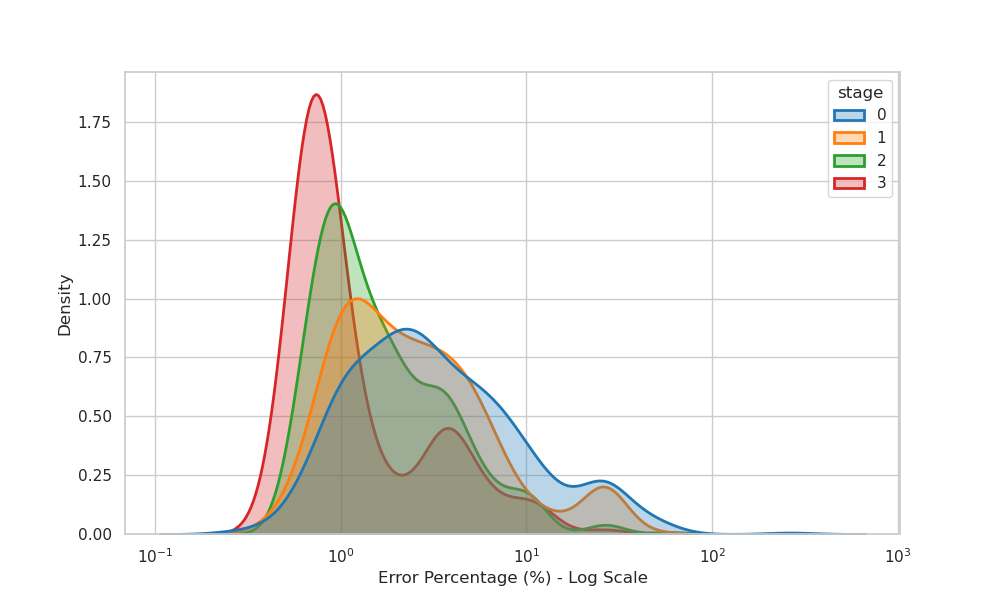
\includegraphics[width=\textwidth]{3-SLAM/3-results/figures/glim_error_distribution_by_stage_log.png}
         \caption{Baseline GLIM tuning.}
         \label{fig:baseline_error_dist}
     \end{subfigure}
     
     \vspace{1em}
     
     \begin{subfigure}[b]{0.8\textwidth}
         \centering
         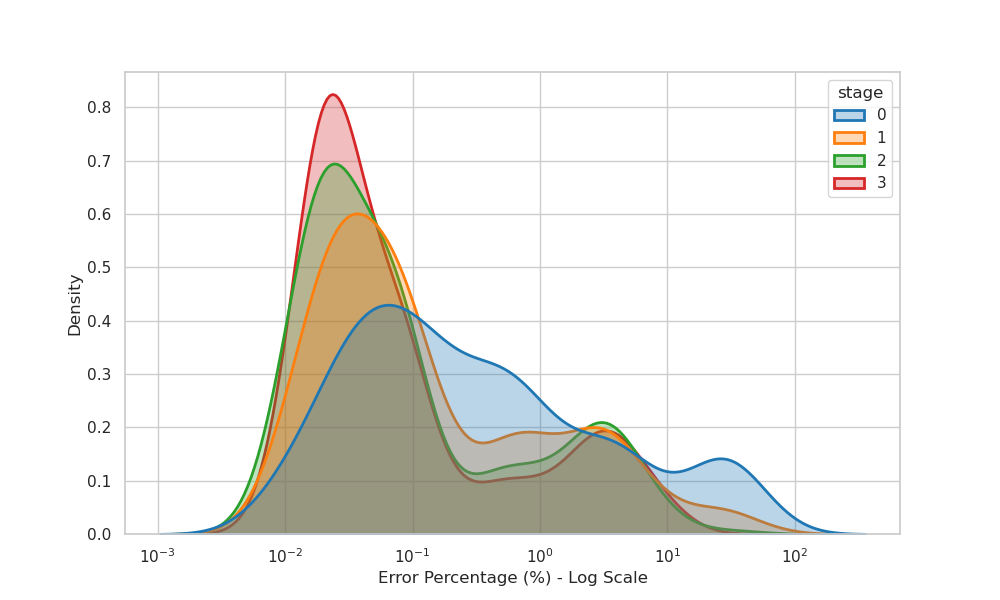
\includegraphics[width=\textwidth]{3-SLAM/3-results/figures/proposed_error_distribution_by_stage_log.png}
         \caption{GLIM-GNSS tuning.}
         \label{fig:proposed_error_dist}
     \end{subfigure}
     
     \caption{Error distribution (log scale) over optimisation stages for baseline tuning (error = error percentage) and GLIM-GNSS tuning (error = GASP).}
     \label{fig:comparison_dist}
\end{figure}

\cref{fig:comparison_progression} plots the best consensus error at the end of each optimisation stage. \cref{fig:baseline_progression} tracks the error percentage for the baseline GLIM, and \cref{fig:proposed_progression} tracks the GASP metric for GLIM-GNSS.

\begin{figure}[htbp]
     \centering
     \begin{subfigure}[b]{0.8\textwidth}
         \centering
         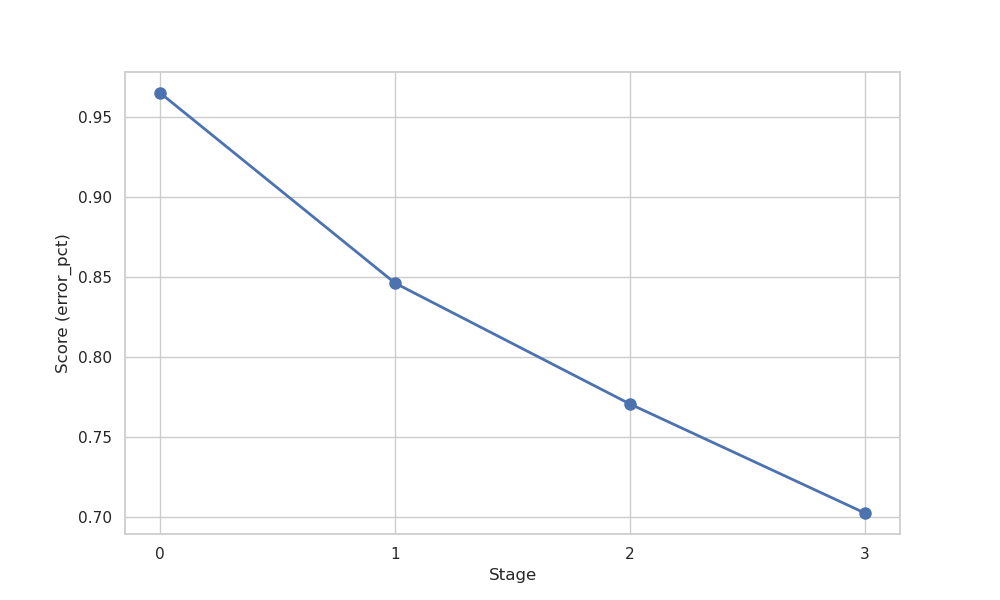
\includegraphics[width=\textwidth]{3-SLAM/3-results/figures/glim_consensus_progression.png}
         \caption{Baseline GLIM error percentage.}
         \label{fig:baseline_progression}
     \end{subfigure}

     \vspace{1.5em}

     \begin{subfigure}[b]{0.8\textwidth}
         \centering
         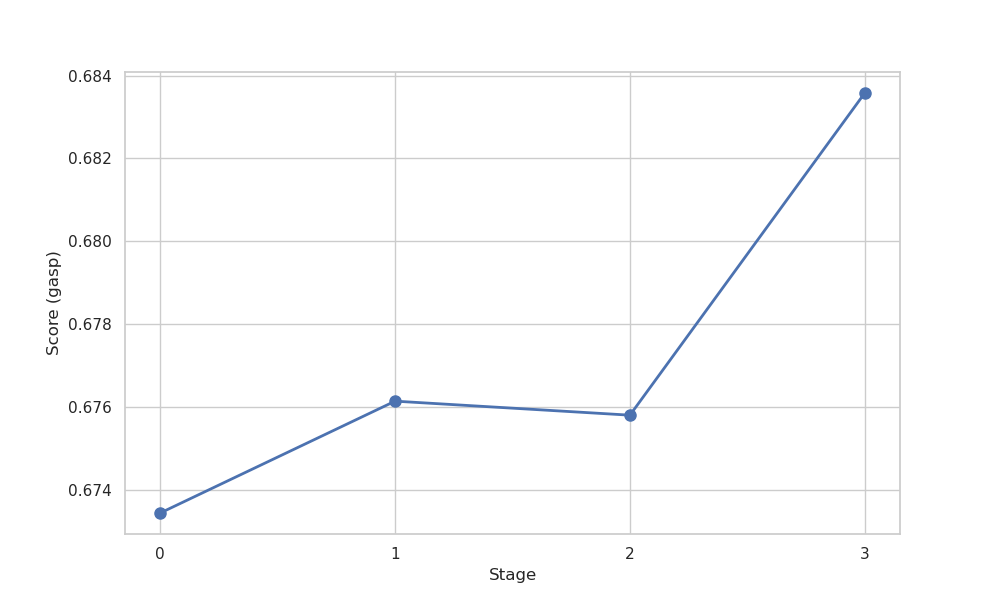
\includegraphics[width=\textwidth]{3-SLAM/3-results/figures/proposed_consensus_progression.png}
         \caption{GLIM-GNSS GASP error.}
         \label{fig:proposed_progression}
     \end{subfigure}
     
     \caption{Consensus error over optimisation stages for baseline tuning (error = error percentage) and GLIM-GNSS tuning (error = GASP).}
     \label{fig:comparison_progression}
\end{figure}

% ===== SLAM: Trajectory Grids =====
\section{SLAM Trajectory Visualisations}
\label{app:slam-trajectory-figures}

\cref{fig:large_grid_xy} presents the planar ($x$--$y$) trajectories for each dataset. The left column shows the refined GLIM output and the right column shows GLIM-GNSS output, both plotted against the RTK~GNSS ground truth.

\begin{figure}[htbp]
    \centering
    % --- ROW 1 ---
    \begin{subfigure}[b]{0.48\textwidth}
        \centering
        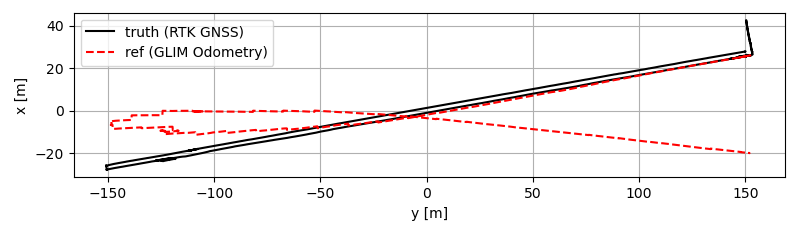
\includegraphics[width=\textwidth]{3-SLAM/3-results/figures/ds0_xy.png}
        \caption{Baseline | Dataset 0}
        \label{fig:ds0_xy_baseline}
    \end{subfigure}
    \hfill
    \begin{subfigure}[b]{0.48\textwidth}
        \centering
        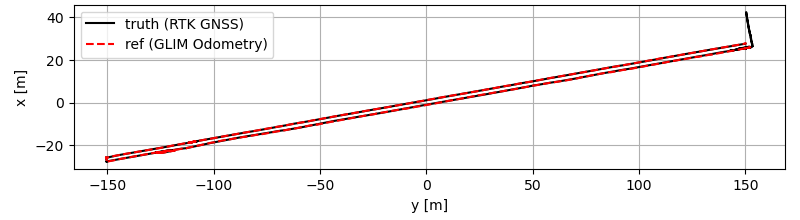
\includegraphics[width=\textwidth]{3-SLAM/3-results/figures/pds0_xy.png}
        \caption{GLIM-GNSS | Dataset 0}
    \end{subfigure}

    \vspace{1em}

    % --- ROW 2 ---
    \begin{subfigure}[b]{0.48\textwidth}
        \centering
        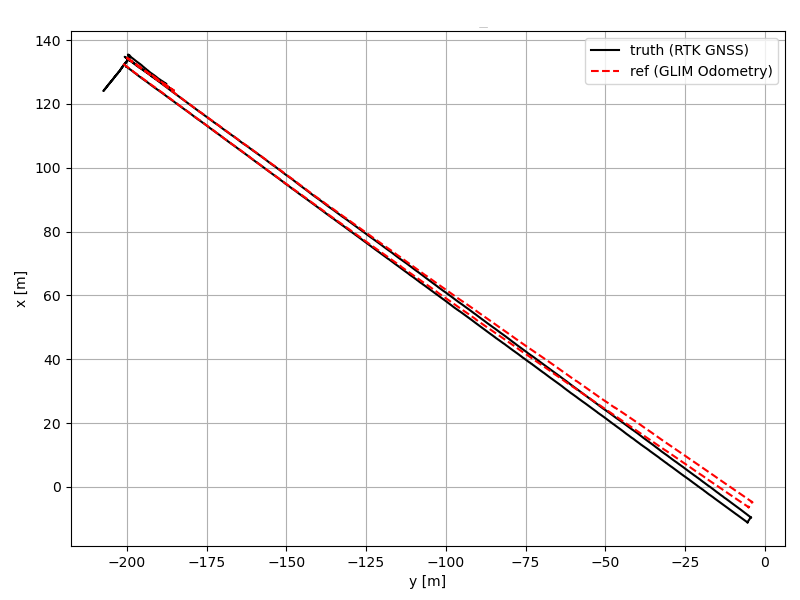
\includegraphics[width=\textwidth]{3-SLAM/3-results/figures/ds1_xy.png}
        \caption{Baseline | Dataset 1}
    \end{subfigure}
    \hfill
    \begin{subfigure}[b]{0.48\textwidth}
        \centering
        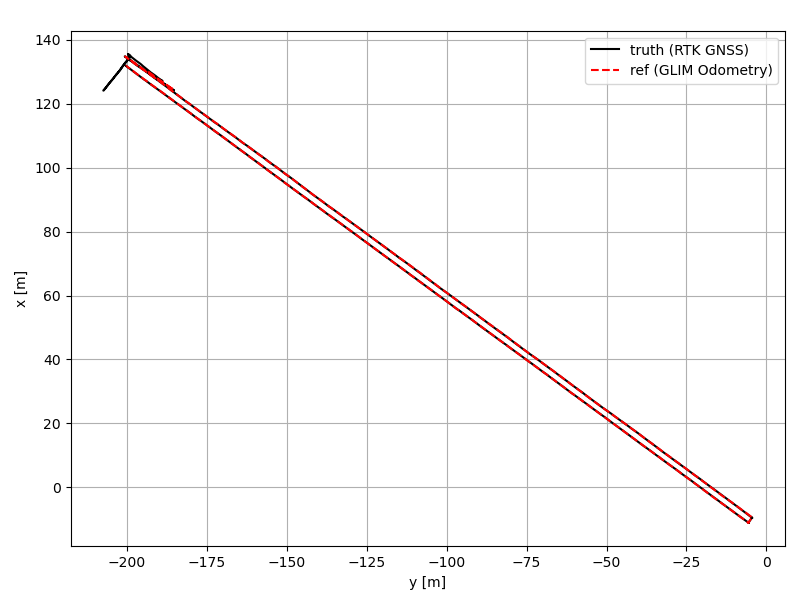
\includegraphics[width=\textwidth]{3-SLAM/3-results/figures/pds1_xy.png}
        \caption{GLIM-GNSS | Dataset 1}
    \end{subfigure}

    \vspace{1em}

    % --- ROW 3 ---
    \begin{subfigure}[b]{0.48\textwidth}
        \centering
        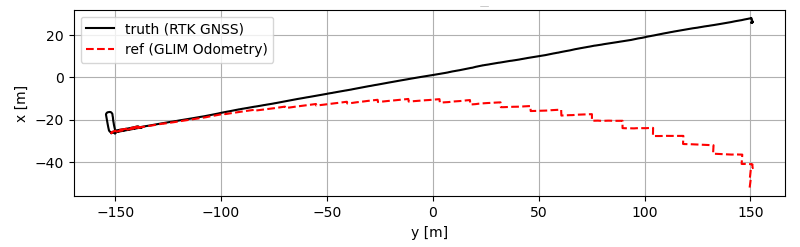
\includegraphics[width=\textwidth]{3-SLAM/3-results/figures/ds2_xy.png}
        \caption{Baseline | Dataset 2}
    \end{subfigure}
    \hfill
    \begin{subfigure}[b]{0.48\textwidth}
        \centering
        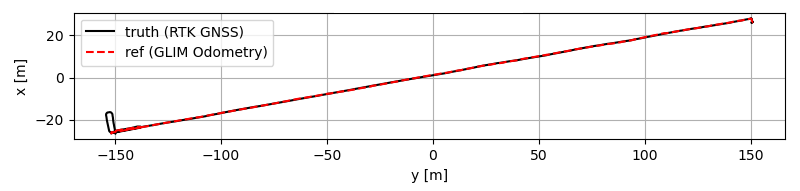
\includegraphics[width=\textwidth]{3-SLAM/3-results/figures/pds2_xy.png}
        \caption{GLIM-GNSS | Dataset 2}
    \end{subfigure}

    \vspace{1em}

    % --- ROW 4 ---
    \begin{subfigure}[b]{0.48\textwidth}
        \centering
        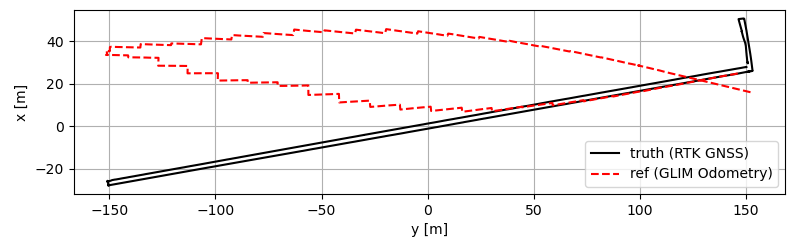
\includegraphics[width=\textwidth]{3-SLAM/3-results/figures/ds3_xy.png}
        \caption{Baseline | Dataset 3}
    \end{subfigure}
    \hfill
    \begin{subfigure}[b]{0.48\textwidth}
        \centering
        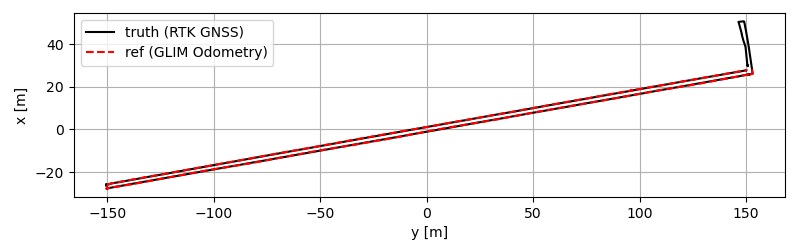
\includegraphics[width=\textwidth]{3-SLAM/3-results/figures/pds3_xy.png}
        \caption{GLIM-GNSS | Dataset 3}
    \end{subfigure}

    \vspace{1em}

    % --- ROW 5 ---
    \begin{subfigure}[b]{0.48\textwidth}
        \centering
        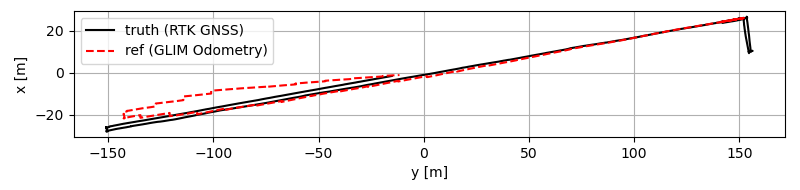
\includegraphics[width=\textwidth]{3-SLAM/3-results/figures/ds4_xy.png}
        \caption{Baseline | Dataset 4}
    \end{subfigure}
    \hfill
    \begin{subfigure}[b]{0.48\textwidth}
        \centering
        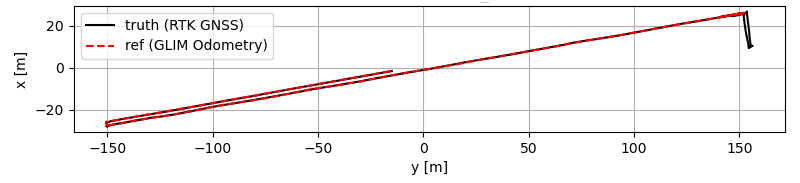
\includegraphics[width=\textwidth]{3-SLAM/3-results/figures/pds4_xy.png}
        \caption{GLIM-GNSS | Dataset 4}
    \end{subfigure}

    \caption{Trajectories in XY plane from baseline GLIM and GLIM-GNSS.}
    \label{fig:large_grid_xy}
\end{figure}

\cref{fig:large_grid_z} presents the altitude ($z$-axis) trajectories for each dataset in the same layout, with the refined GLIM estimates on the left and GLIM-GNSS estimates on the right, both compared against RTK~GNSS ground truth.

\begin{figure}[htbp]
    \centering
    % --- ROW 1 ---
    \begin{subfigure}[b]{0.48\textwidth}
        \centering
        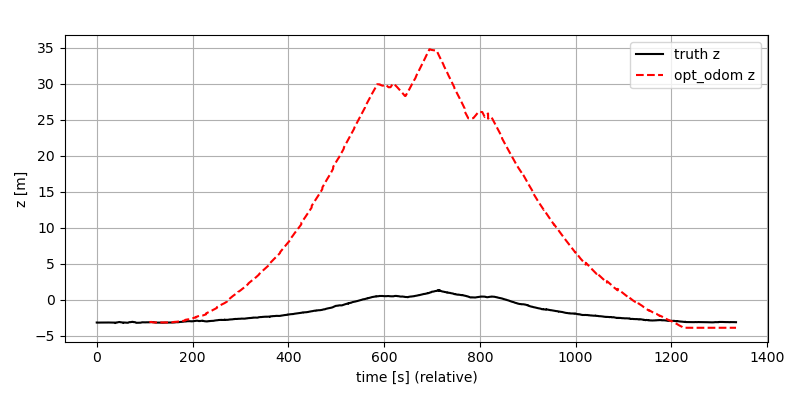
\includegraphics[width=\textwidth]{3-SLAM/3-results/figures/ds0_z.png}
        \caption{Baseline | Dataset 0}
    \end{subfigure}
    \hfill
    \begin{subfigure}[b]{0.48\textwidth}
        \centering
        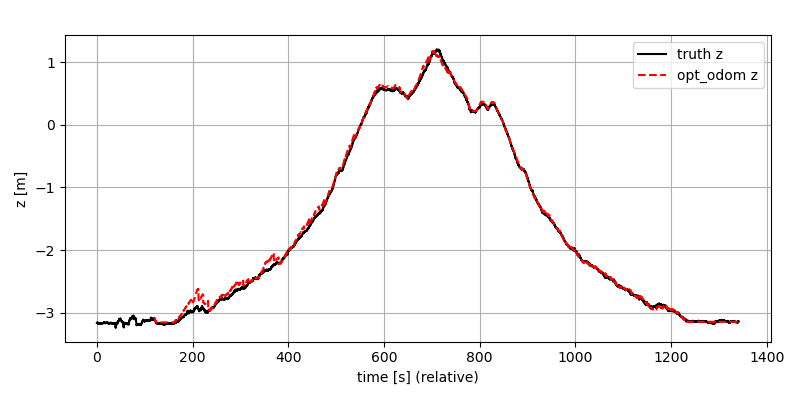
\includegraphics[width=\textwidth]{3-SLAM/3-results/figures/pds0_z.png}
        \caption{GLIM-GNSS | Dataset 0}
    \end{subfigure}

    \vspace{1em}

    % --- ROW 2 ---
    \begin{subfigure}[b]{0.48\textwidth}
        \centering
        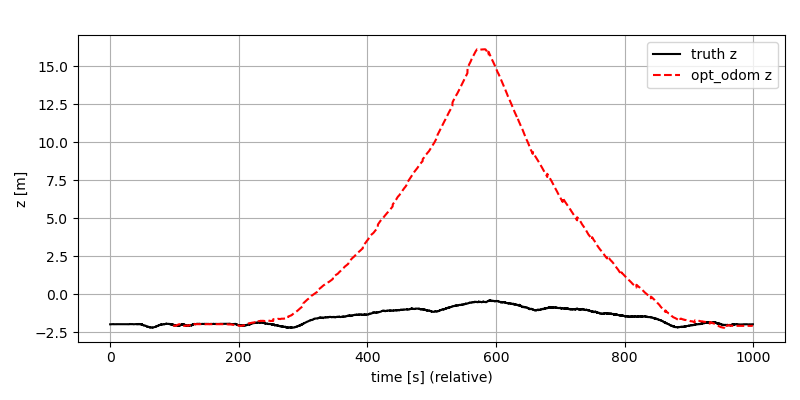
\includegraphics[width=\textwidth]{3-SLAM/3-results/figures/ds1_z.png}
        \caption{Baseline | Dataset 1}
    \end{subfigure}
    \hfill
    \begin{subfigure}[b]{0.48\textwidth}
        \centering
        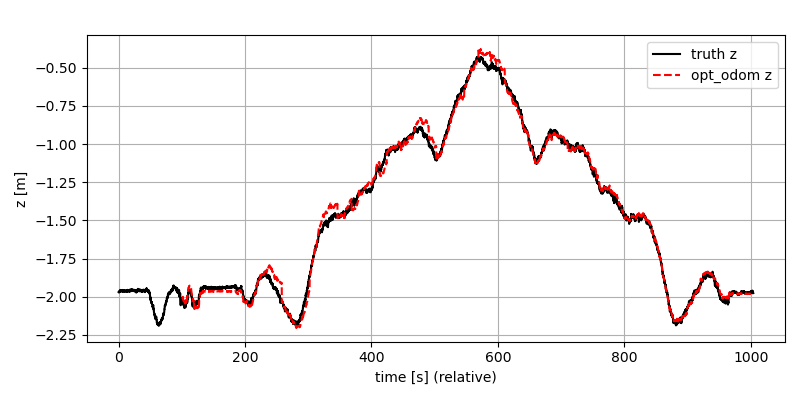
\includegraphics[width=\textwidth]{3-SLAM/3-results/figures/pds1_z.png}
        \caption{GLIM-GNSS | Dataset 1}
    \end{subfigure}

    \vspace{1em}

    % --- ROW 3 ---
    \begin{subfigure}[b]{0.48\textwidth}
        \centering
        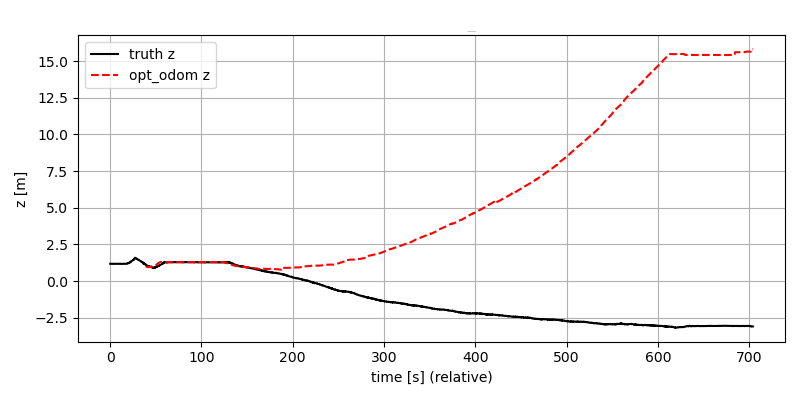
\includegraphics[width=\textwidth]{3-SLAM/3-results/figures/ds2_z.png}
        \caption{Baseline | Dataset 2}
    \end{subfigure}
    \hfill
    \begin{subfigure}[b]{0.48\textwidth}
        \centering
        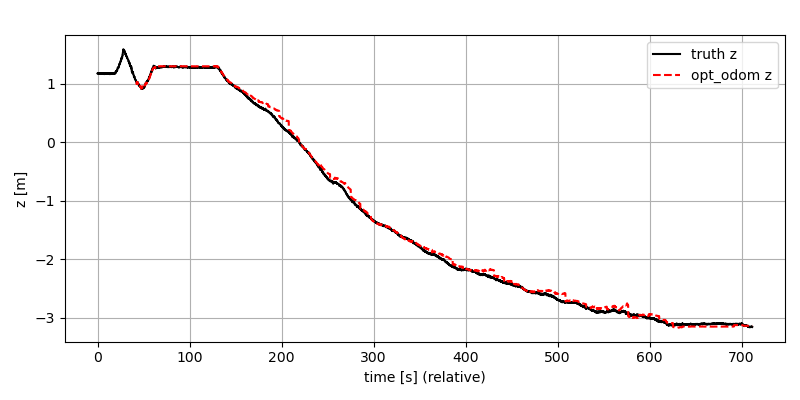
\includegraphics[width=\textwidth]{3-SLAM/3-results/figures/pds2_z.png}
        \caption{GLIM-GNSS | Dataset 2}
    \end{subfigure}

    \vspace{1em}

    % --- ROW 4 ---
    \begin{subfigure}[b]{0.48\textwidth}
        \centering
        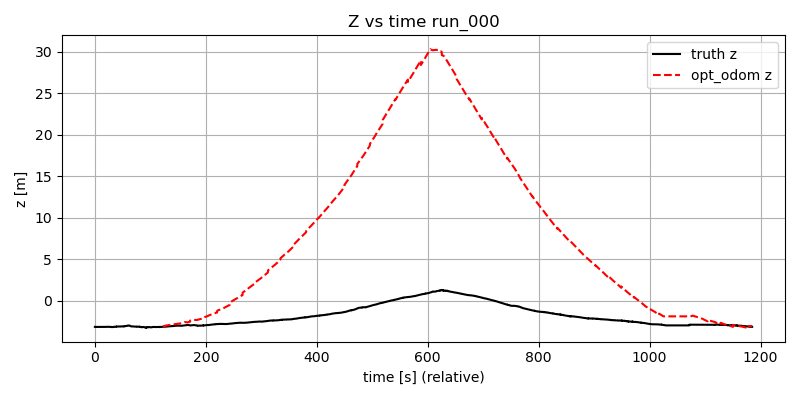
\includegraphics[width=\textwidth]{3-SLAM/3-results/figures/ds3_z.png}
        \caption{Baseline | Dataset 3}
    \end{subfigure}
    \hfill
    \begin{subfigure}[b]{0.48\textwidth}
        \centering
        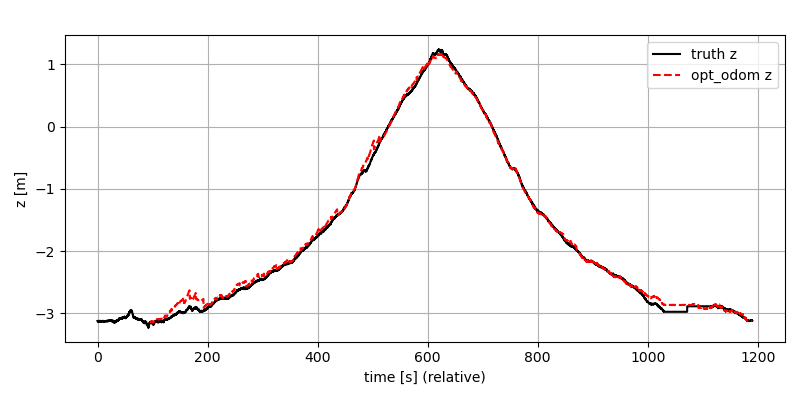
\includegraphics[width=\textwidth]{3-SLAM/3-results/figures/pds3_z.png}
        \caption{GLIM-GNSS | Dataset 3}
    \end{subfigure}

    \vspace{1em}

    % --- ROW 5 ---
    \begin{subfigure}[b]{0.48\textwidth}
        \centering
        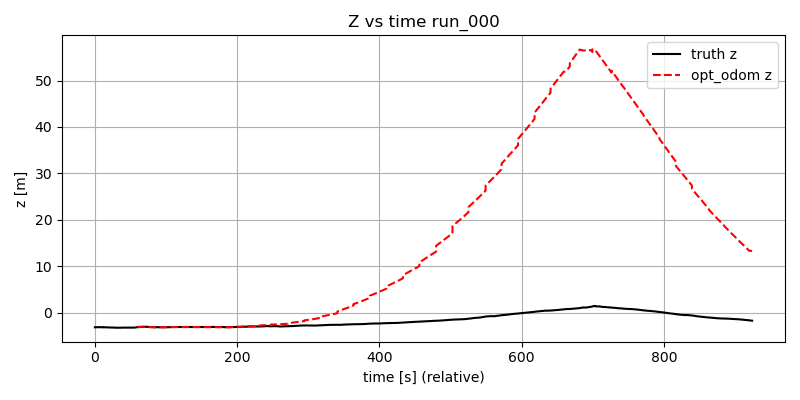
\includegraphics[width=\textwidth]{3-SLAM/3-results/figures/ds4_z.png}
        \caption{Baseline | Dataset 4}
        \label{fig:ds4_z_baseline}
    \end{subfigure}
    \hfill
    \begin{subfigure}[b]{0.48\textwidth}
        \centering
        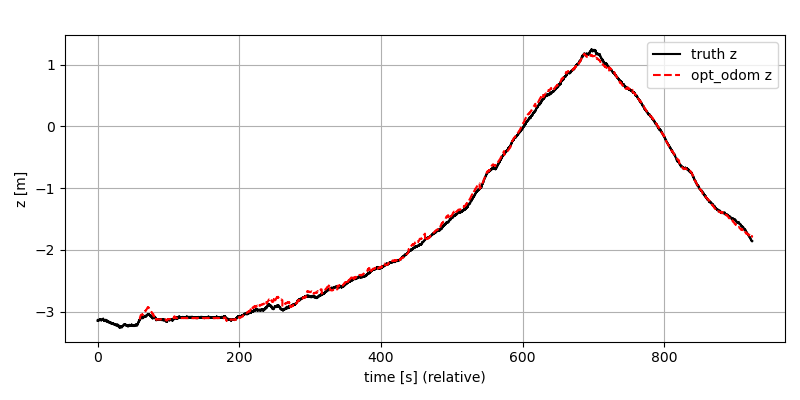
\includegraphics[width=\textwidth]{3-SLAM/3-results/figures/pds4_z.png}
        \caption{GLIM-GNSS | Dataset 4}
    \end{subfigure}

    \caption{Trajectories in Z plane from baseline GLIM and GLIM-GNSS.}
    \label{fig:large_grid_z}
\end{figure}

% ===== Precise Alignment: LiDAR Heatmap =====
\section{Precise Alignment Supplementary Figures}
\label{app:pa-supplementary-figures}

\begin{figure}[htbp]
  \centering
  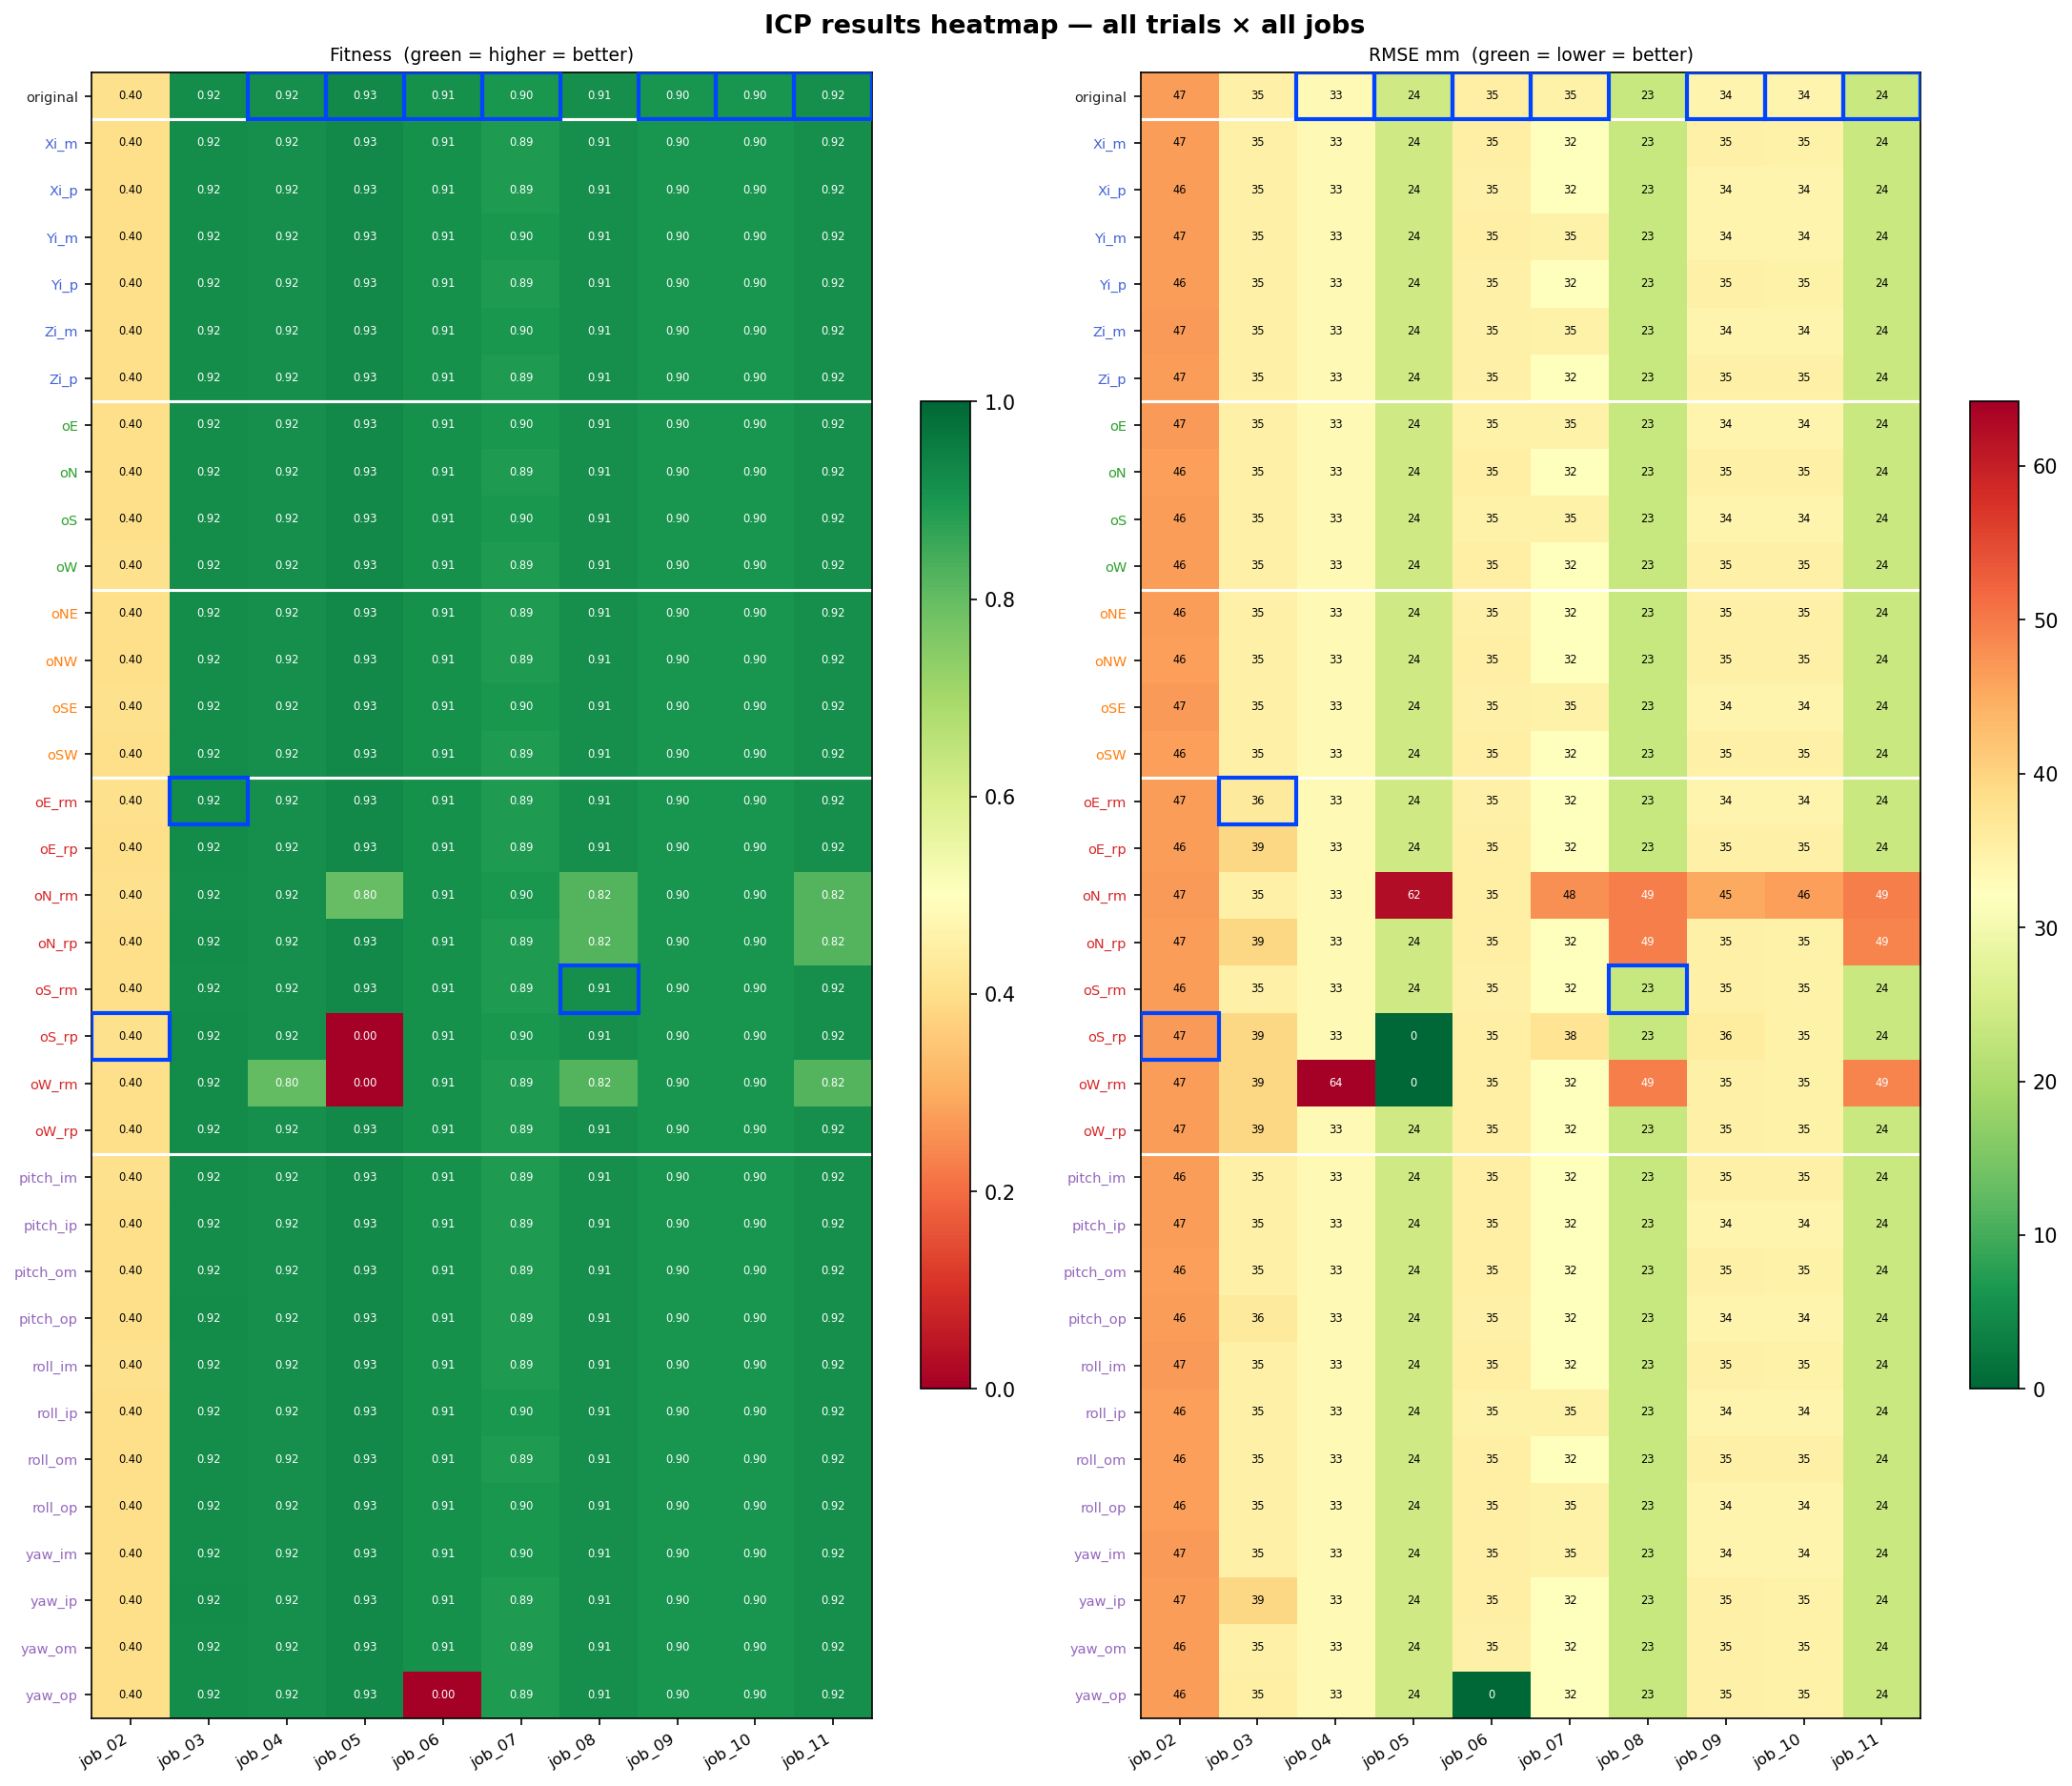
\includegraphics[width=\linewidth]{4-precise-alignment/4-results/figures/lidar_icp_heatmap}
  \caption{ICP fitness heatmap across all 315 LiDAR hypotheses. Each row corresponds to one condition (ordered by distance); each column to one perturbation hypothesis. Colour intensity indicates fitness score. The D110A0 row was excluded from analysis as it exceeded the stereo pipeline's depth clipping threshold.}
  \label{fig:pa-lidar-heatmap}
\end{figure}

\begin{figure}[htbp]
  \centering
  \begin{subfigure}[b]{0.32\linewidth}
    \centering
    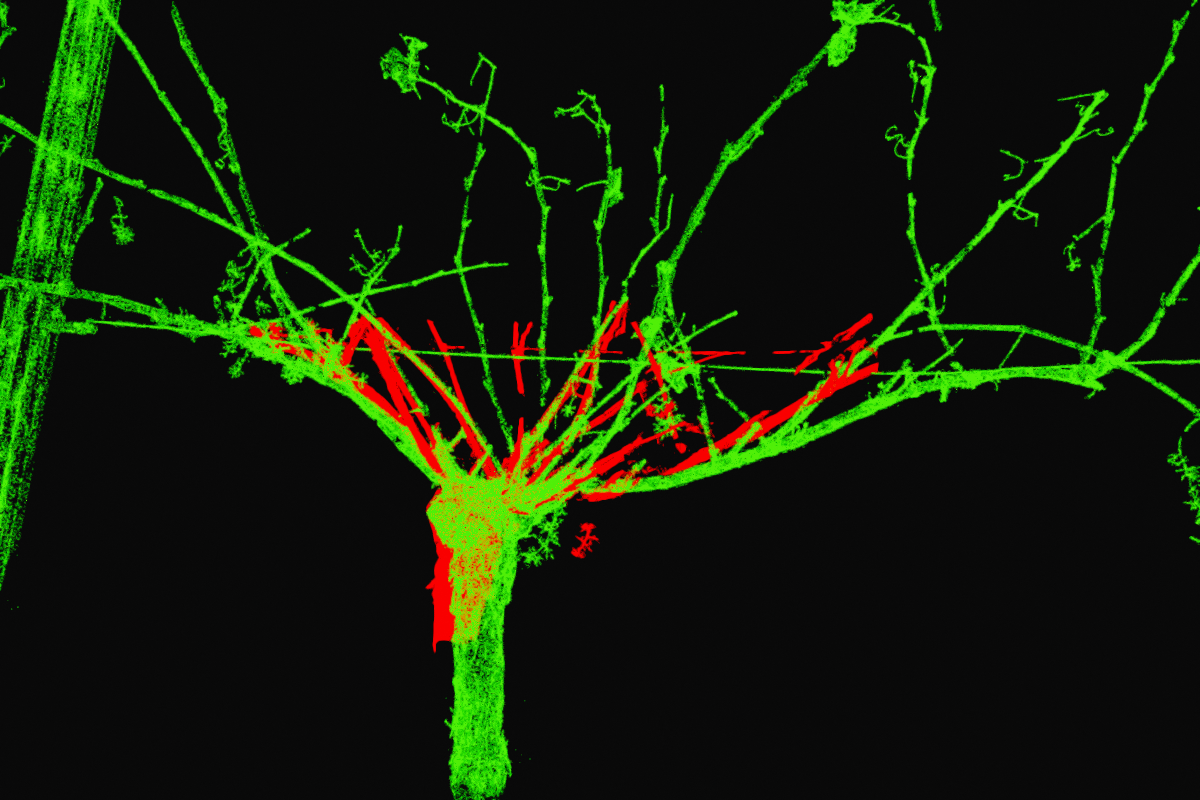
\includegraphics[width=\linewidth]{4-precise-alignment/4-results/figures/stereo_D40Am15_5b_icp_final_side}
    \caption{D40A$-$15}
  \end{subfigure}
  \hfill
  \begin{subfigure}[b]{0.32\linewidth}
    \centering
    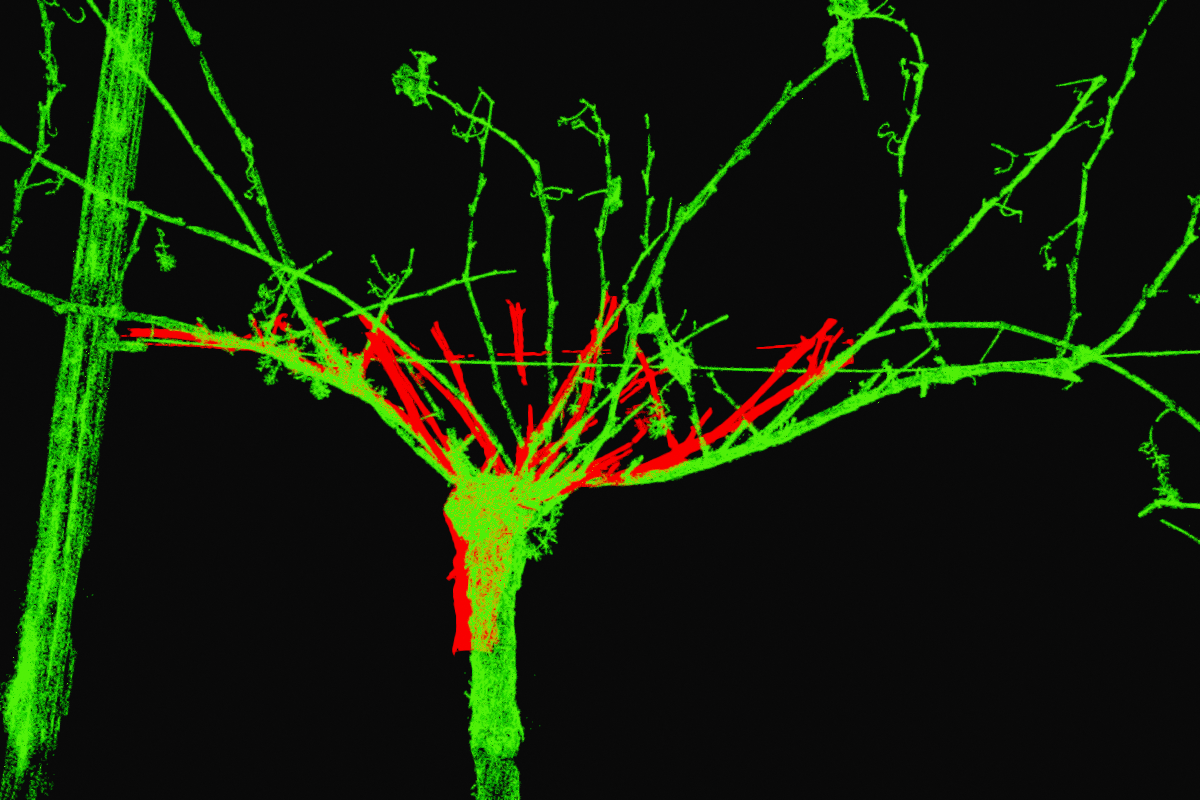
\includegraphics[width=\linewidth]{4-precise-alignment/4-results/figures/stereo_D40A0_5b_icp_final_side}
    \caption{D40A0}
  \end{subfigure}
  \hfill
  \begin{subfigure}[b]{0.32\linewidth}
    \centering
    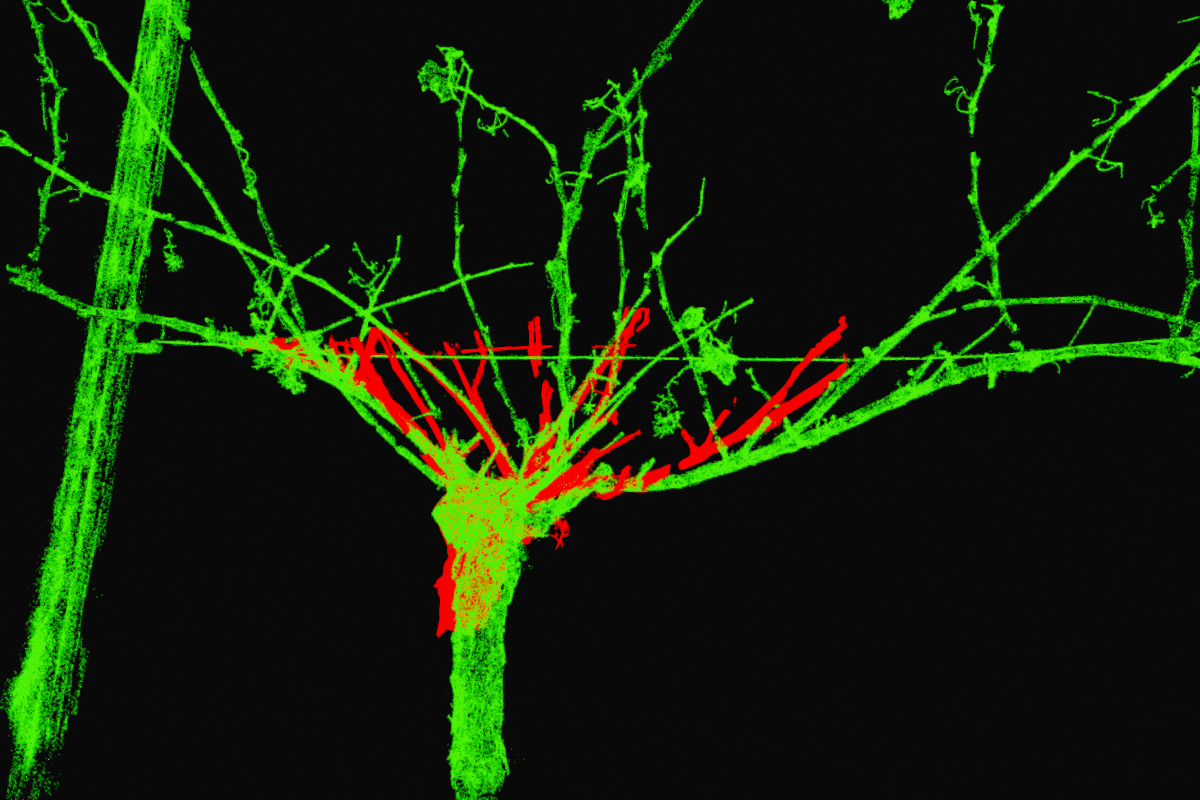
\includegraphics[width=\linewidth]{4-precise-alignment/4-results/figures/stereo_D60Am15_5b_icp_final_side}
    \caption{D60A$-$15}
  \end{subfigure}

  \vspace{0.5em}

  \begin{subfigure}[b]{0.32\linewidth}
    \centering
    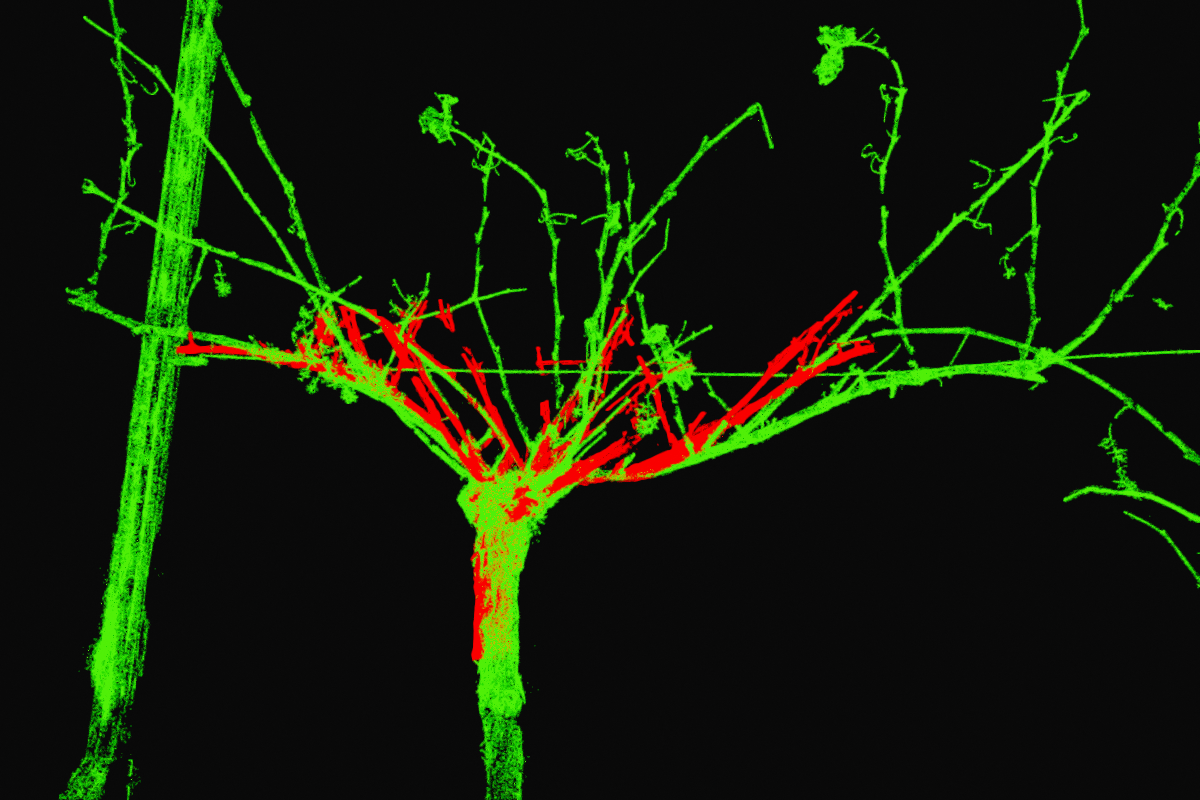
\includegraphics[width=\linewidth]{4-precise-alignment/4-results/figures/stereo_D60A0_5b_icp_final_side}
    \caption{D60A0}
  \end{subfigure}
  \hfill
  \begin{subfigure}[b]{0.32\linewidth}
    \centering
    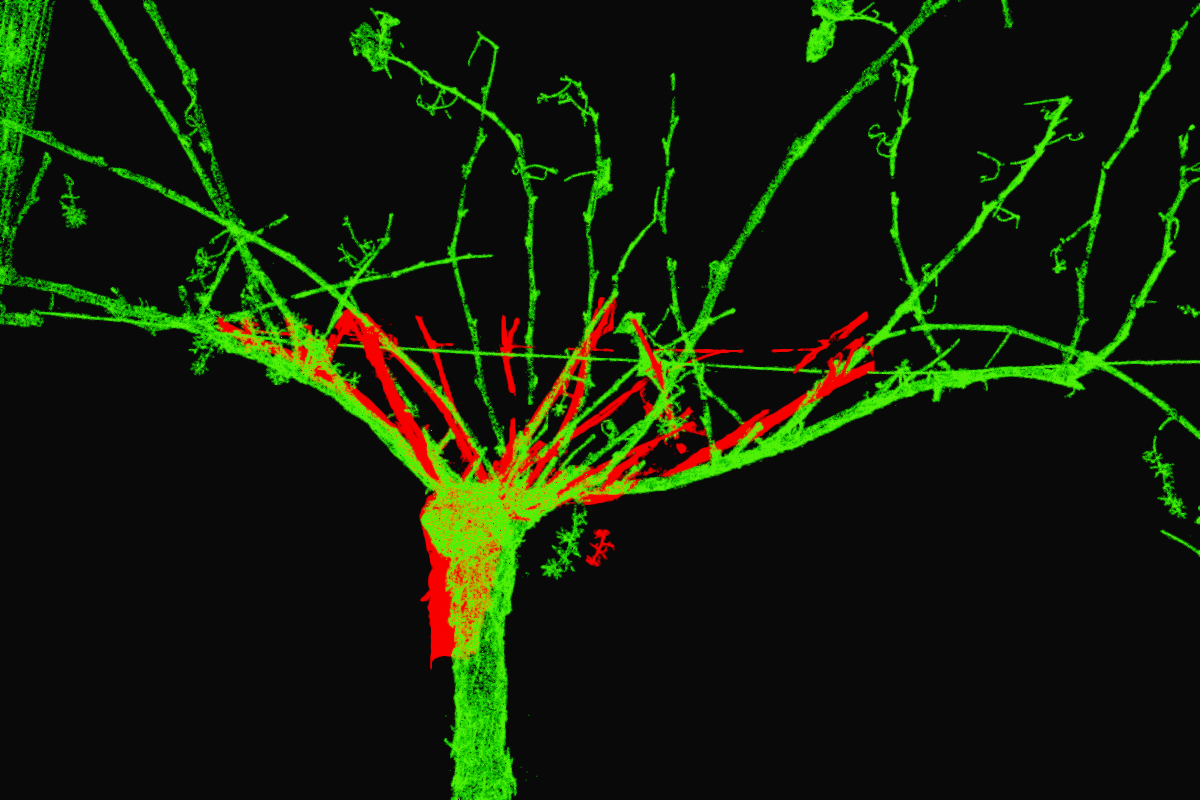
\includegraphics[width=\linewidth]{4-precise-alignment/4-results/figures/stereo_D60Ap15_5b_icp_final_side}
    \caption{D60A$+$15}
  \end{subfigure}
  \hfill
  \begin{subfigure}[b]{0.32\linewidth}
    \centering
    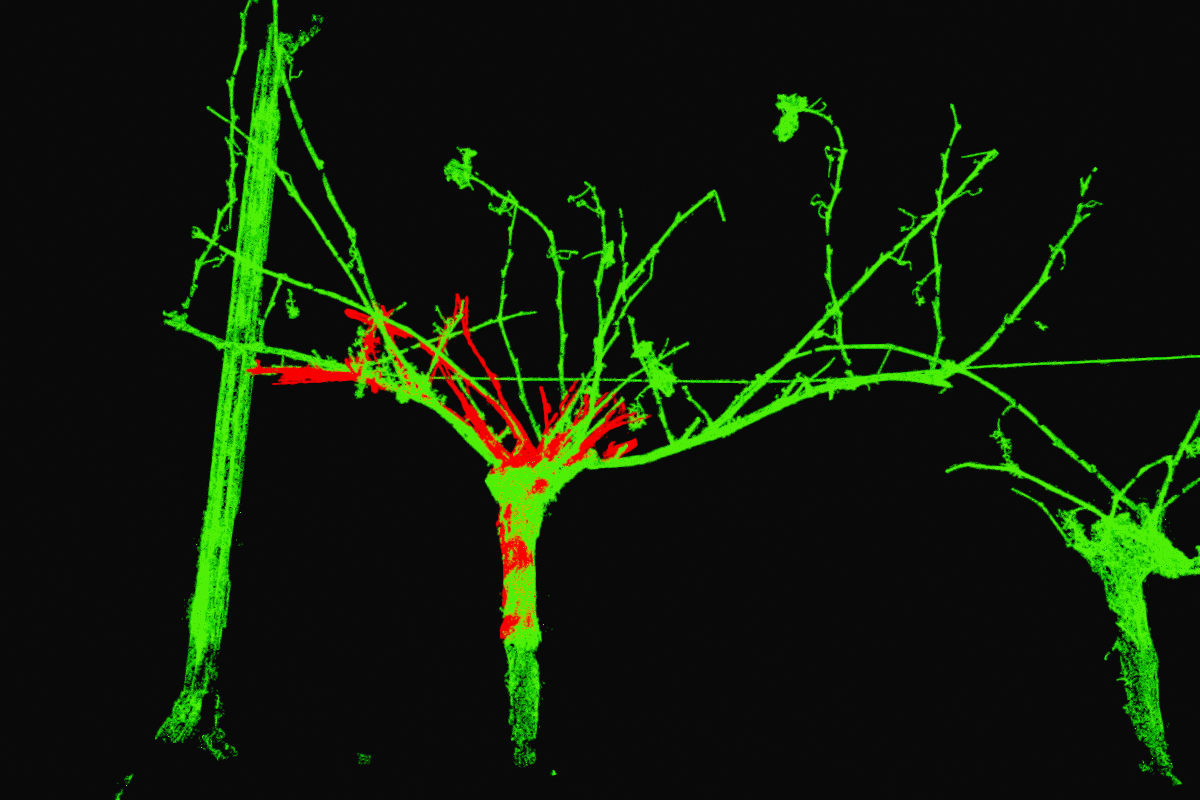
\includegraphics[width=\linewidth]{4-precise-alignment/4-results/figures/stereo_D80A0_5b_icp_final_side}
    \caption{D80A0}
  \end{subfigure}

  \vspace{0.5em}

  \begin{subfigure}[b]{0.32\linewidth}
    \centering
    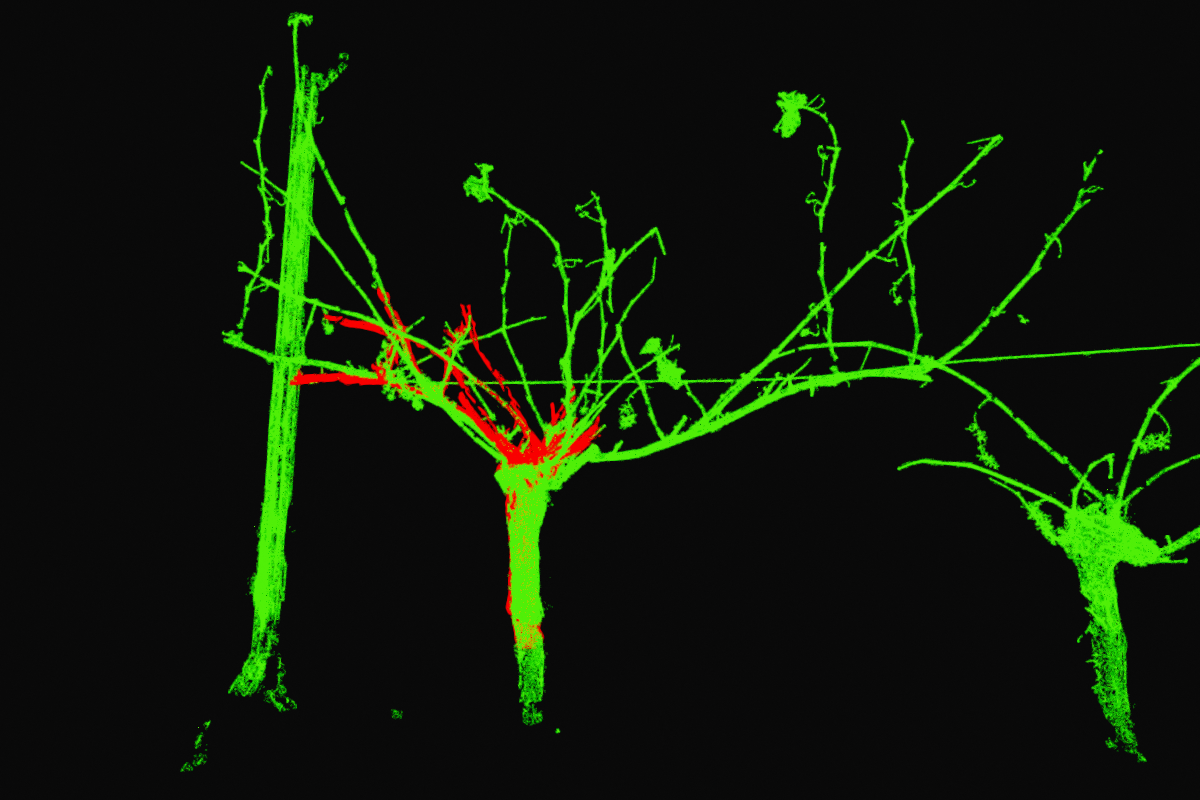
\includegraphics[width=\linewidth]{4-precise-alignment/4-results/figures/stereo_D80Ap15_5b_icp_final_side}
    \caption{D80A$+$15}
  \end{subfigure}
  \caption{Final stereo ICP alignment (vine-face view) for all seven converging conditions. Green: 3DGS reference cloud; red: registered stereo source cloud.}
  \label{fig:pa-stereo-converged-overlay}
\end{figure}